%----------------------------------------------------------------------------------------
%	PACKAGES AND THEMES
%----------------------------------------------------------------------------------------
\documentclass[aspectratio=169,xcolor=dvipsnames]{beamer}
\usetheme{Simple}
\usepackage{mathrsfs,mathtools}
\mathtoolsset{showonlyrefs}

\usepackage{natbib}
\usepackage{dsfont}

\usepackage{hyperref}
\usepackage{graphicx} % Allows including images
\usepackage{booktabs}
\usepackage{multirow}
\usepackage{bm}
\usepackage{tikz}
\def\caliB{\mathscr{B}}

\usepackage[dvipsnames]{xcolor}
\usepackage{caption}
\input macros.tex

\def\caliP{\mathscr{P}_{\textup{sgn}}}

\usepackage{appendixnumberbeamer}
\setbeamertemplate{footline}[frame number]



% Allows the use of \toprule, \midrule and \bottomrule in tables

%----------------------------------------------------------------------------------------
%	TITLE PAGE
%----------------------------------------------------------------------------------------

% The title
\title[short title]{Smooth tensor estimation with unknown permutation}

 \author[Chanwoo] {Chanwoo Lee$^1$ and Miaoyan Wang$^2$}

\institute[UWM] % Your institution may be shorthand to save space
{
    % Your institution for the title page
    Department of Statistics,
    University of Wisconsin - Madison
    \vskip 3pt
    {\scriptsize\let\thefootnote\relax\footnote{\hspace{-.5cm}{$^1$\texttt{chanwoo.lee@wisc.edu} $^2$\texttt{miaoyan.wang@wisc.edu}}
    }}

}

\date{NeurIPS workshop on Quantum Tensor Networks in Machine Learning} % Date, can be changed to a custom date


%----------------------------------------------------------------------------------------
%	PRESENTATION SLIDES
%----------------------------------------------------------------------------------------

\begin{document}

\AtBeginSubsection[]{%
  \frame<beamer>{ 
    \frametitle{Outline}   
    \tableofcontents[currentsection,currentsubsection] 
  }
}

\begin{frame}
    % Print the title page as the first slide
    \titlepage
\end{frame}



%------------------------------------------------
%------------------------------------------------





% \begin{frame}{What is tensor?}
%     \begin{itemize}
%         \item Tensors are generalizations of vectors and matrices:
%         \begin{center}
%             \includegraphics[width=9cm]{figure/tensorimage.png}
%         \end{center}
%          \item We focus on tensors of order 3 or greater, also called {\color{red}{higher-order tensors.} }
%         \item Denote an order-$K (d_1,\cdots,d_K)$ dimensional tensor as $\mathcal{Y} = \entry{y_\omega}\in\mathbb{R}^{d_1\times\cdots\times d_K}$ \\
%         where $\omega \in [d_1]\times \cdots\times [d_K].$
%     \end{itemize}
% \end{frame}

% \begin{frame}{Tensors in application}
%   \begin{center}
%     \includegraphics[width =\textwidth]{figure/ndataset.pdf}
%     \end{center}
%     \begin{enumerate}
    
%      \item The human brain connectivity dataset consists of 68 brain regions for 114 individuals~\citep{wang2017bayesian}.

%  \item The NIPS dataset consists of word occurrence counts in papers published from 1987 to 2003  along with author information~\citep{globerson2007euclidean}.

%  \item An RGB image consists of pixel values across three channels.
%     \end{enumerate}
% \end{frame}





\begin{frame}{Main problems: the permuted signal plus noise model}
\begin{center}
    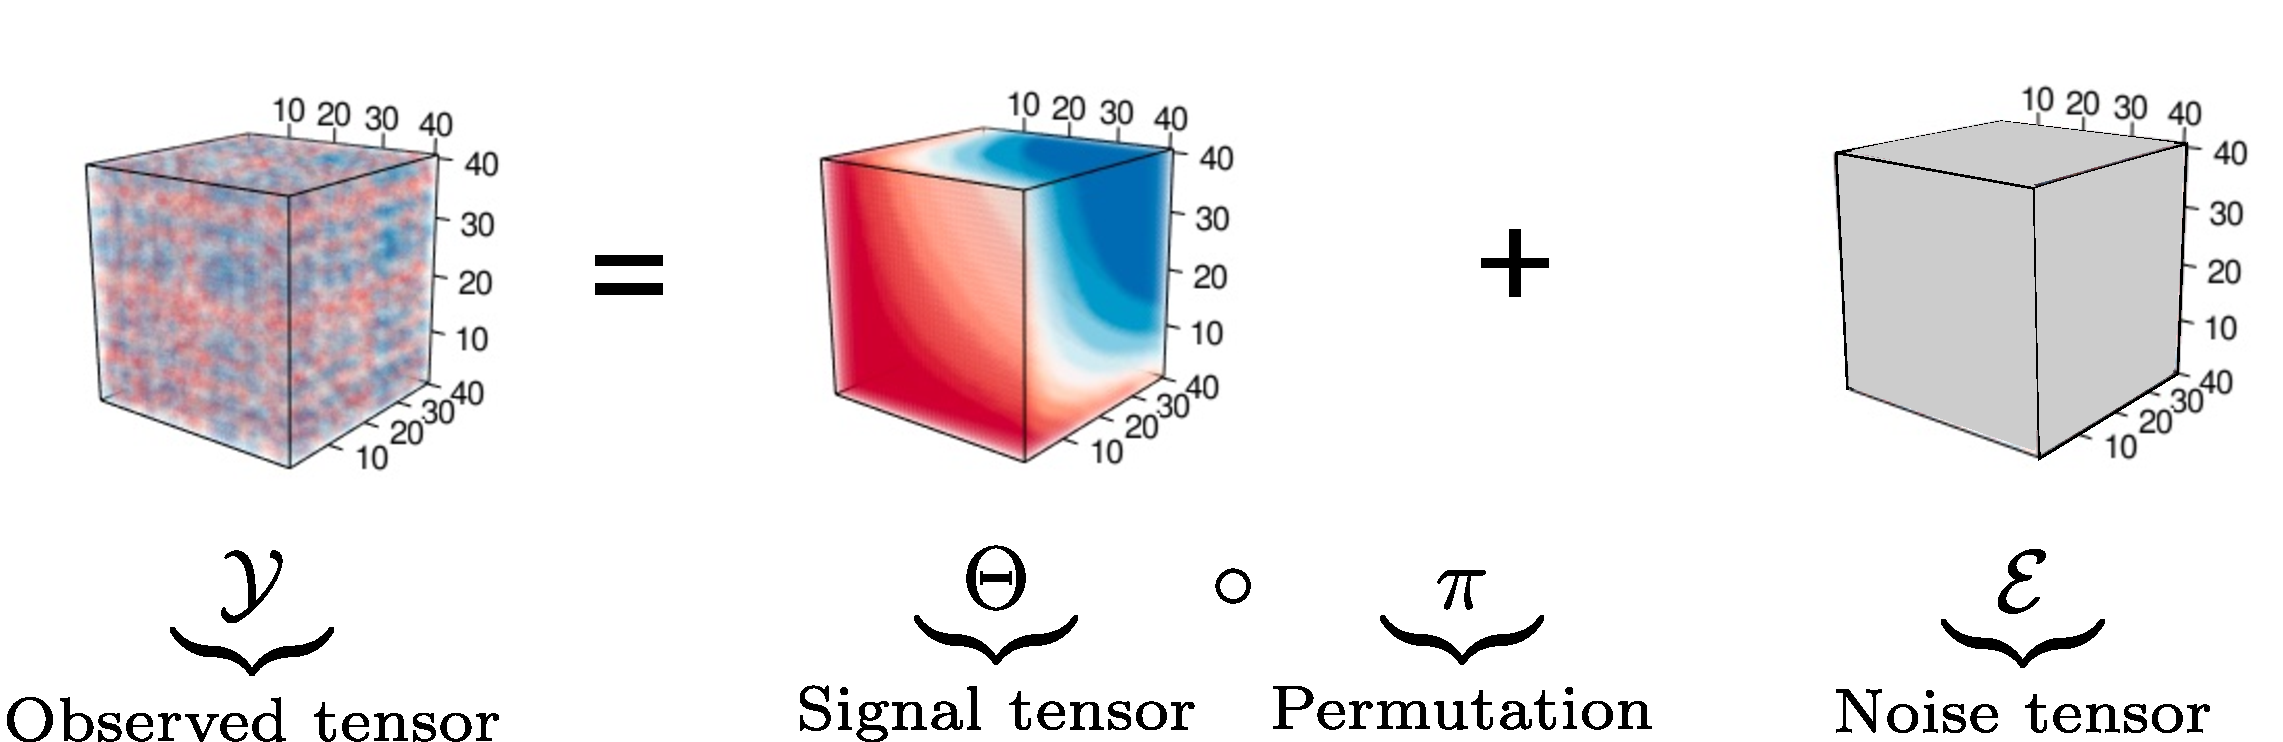
\includegraphics[width = 0.85\textwidth]{figure/spnm.pdf}
\end{center}
\begin{itemize}
    \item 
Question: How to estimate {\color{red}the permuted signal tensor} $\Theta\circ \pi$?
\end{itemize}


\begin{itemize}
  \onslide<2->{
% % \begin{column}{0.6\textwidth}
\item We assume that there exists a {\color{red}multivariate function} $f\colon [0,1]^m\rightarrow \mathbb{R}$ underlying the signal tensor, such that
\begin{align}\label{eq:rep}
\Theta_{i_1,\ldots,i_m} = f\left({i_1\over d},\ldots,{i_m\over d}\right), \text{ for all } i_1,\ldots,i_m\in[d].
\end{align}
% \end{column}
% \begin{column}{0.4\textwidth}
% \begin{figure}
%   \begin{center}
%     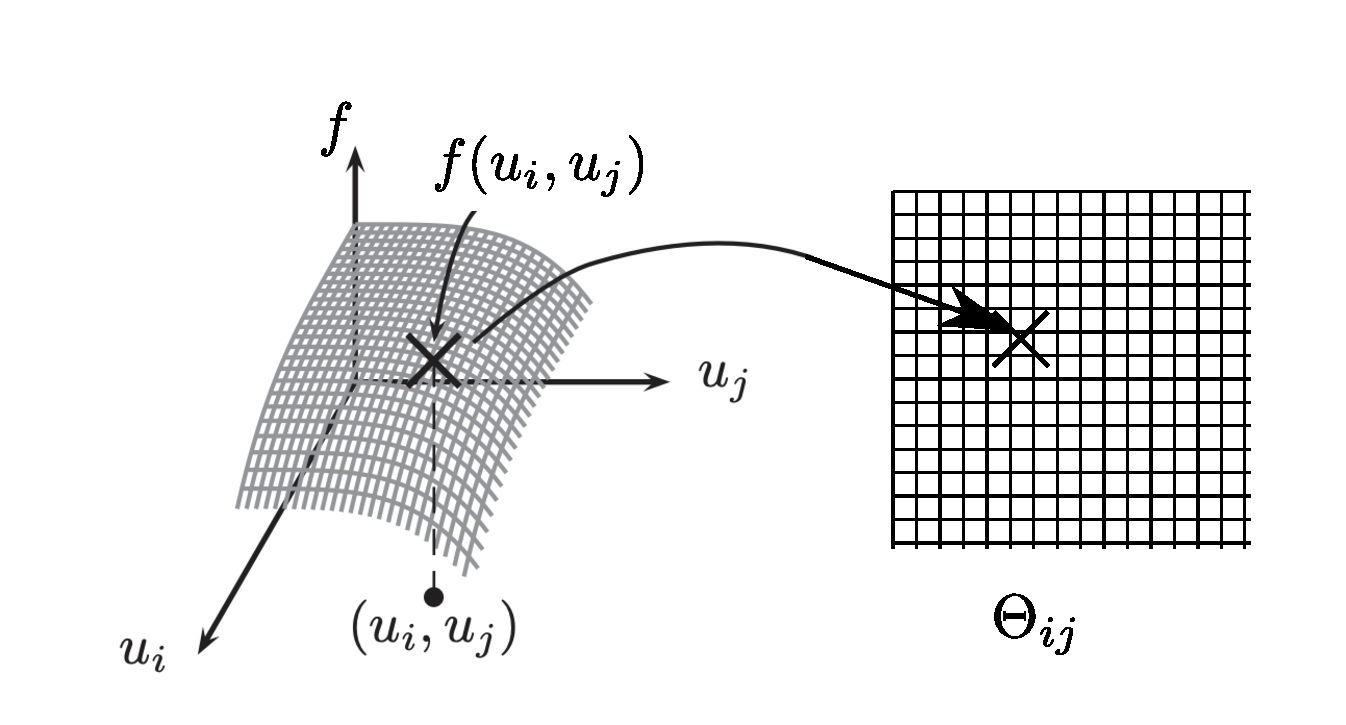
\includegraphics[width =5cm]{figure/fmodel.pdf}
%     \caption*{\scriptsize The figure is adopted from~\cite{airoldi2013stochastic}.}
%     \end{center}
% \end{figure}
% \end{column}
% \end{columns}
}
\end{itemize}

\end{frame}

\begin{frame}{Our contribution}
% \includegraphics[width = \textwidth]{figure/image_new2.pdf}
% Special case with full observation:\\[.5cm]

    \resizebox{\columnwidth}{!}{%
    \begin{tabular}{c|cccc}
    & \cite{pananjady2020isotonic}&  \cite{balasubramanian2021nonparametric}& \cite{li2019nearest}&\textbf{Ours$^*$}\\
    \hline
       model structure& monotonic & Lipschitz & Lipschitz &  $\alpha$-smoothness  \\
     minimax lower bound& $\surd$  & $\times$ & $\times$ & $\surd$ \\
     error rate for order-3 tensors& $d^{-1}$ & $d^{-6/5}$ & $d^{-1}$ & ${\color{red}d^{-2}}$ \\
     polynomial algorithm& $\surd$ &$\times$ & $\surd$ & $\surd$\\
        \hline
    \end{tabular}
}

{\scriptsize \hfill We list here only the result for infinitely smooth order-3 tensors.}

\begin{itemize}
    \item We develop a general permuted model for an arbitrary smoothness and order of tensors with {\color{red}optimal rate}.
\end{itemize}

\onslide<2->{
    \begin{columns}
\begin{column}{0.26\textwidth}
   \begin{center}
     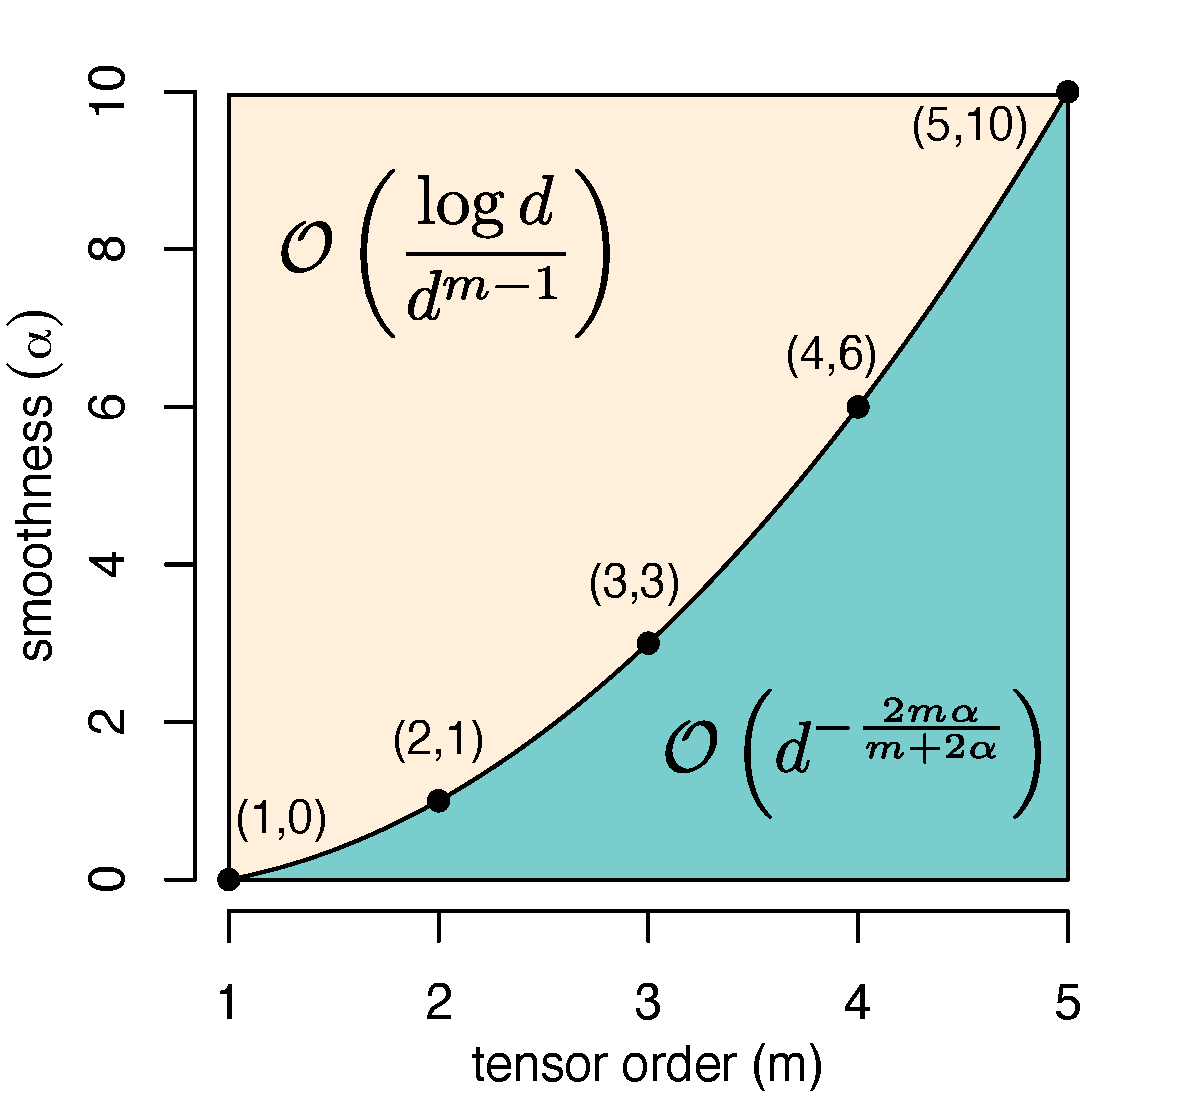
\includegraphics[width=\textwidth]{figure/ratio.pdf}
     \end{center}
\end{column}
\begin{column}{0.7\textwidth} 
\begin{itemize}
    \item We discover a {\color{red}phase transition phenomenon} with respect to the smoothness threshold needed for optimal tensor recovery.
    \item We provide an efficient {\color{red}polynomial-time Borda count algorithm} that provably achieves optimal rate.
\end{itemize}
\end{column}
\end{columns}
}


\end{frame}


% \begin{frame}{Tensor based learning is challenging}
% 	\begin{itemize}
% 	\item {\bf High-rank matrix model} \citep{ganti2015matrix,pmlr-v70-ongie17a,fan2019online}\\[.3cm]
% 		\begin{itemize}
%  \onslide<2->{\item \color{red}Applying matrix methods  to higher-order tensor destroys structural information.\\[.2cm]\item
%  Tensors are more challenging because tensor rank may exceed dimension.}
% \end{itemize}
% 	\end{itemize}
% \vspace*{.5cm}
% \begin{itemize}
% 	\onslide<3->{\item {\bf  Low-rank tensor model}~\citep{anandkumar2014tensor,montanari2018spectral,cai2019nonconvex}\\[.3cm]
% 	\begin{itemize}
% 	    \item {\color{red}Low-rank models are inadequate in many cases.}
% 	\end{itemize}}
% 	\end{itemize}
% \end{frame}

\begin{frame}{Block-wise polynomial approximation}
\begin{figure}
    \centering
    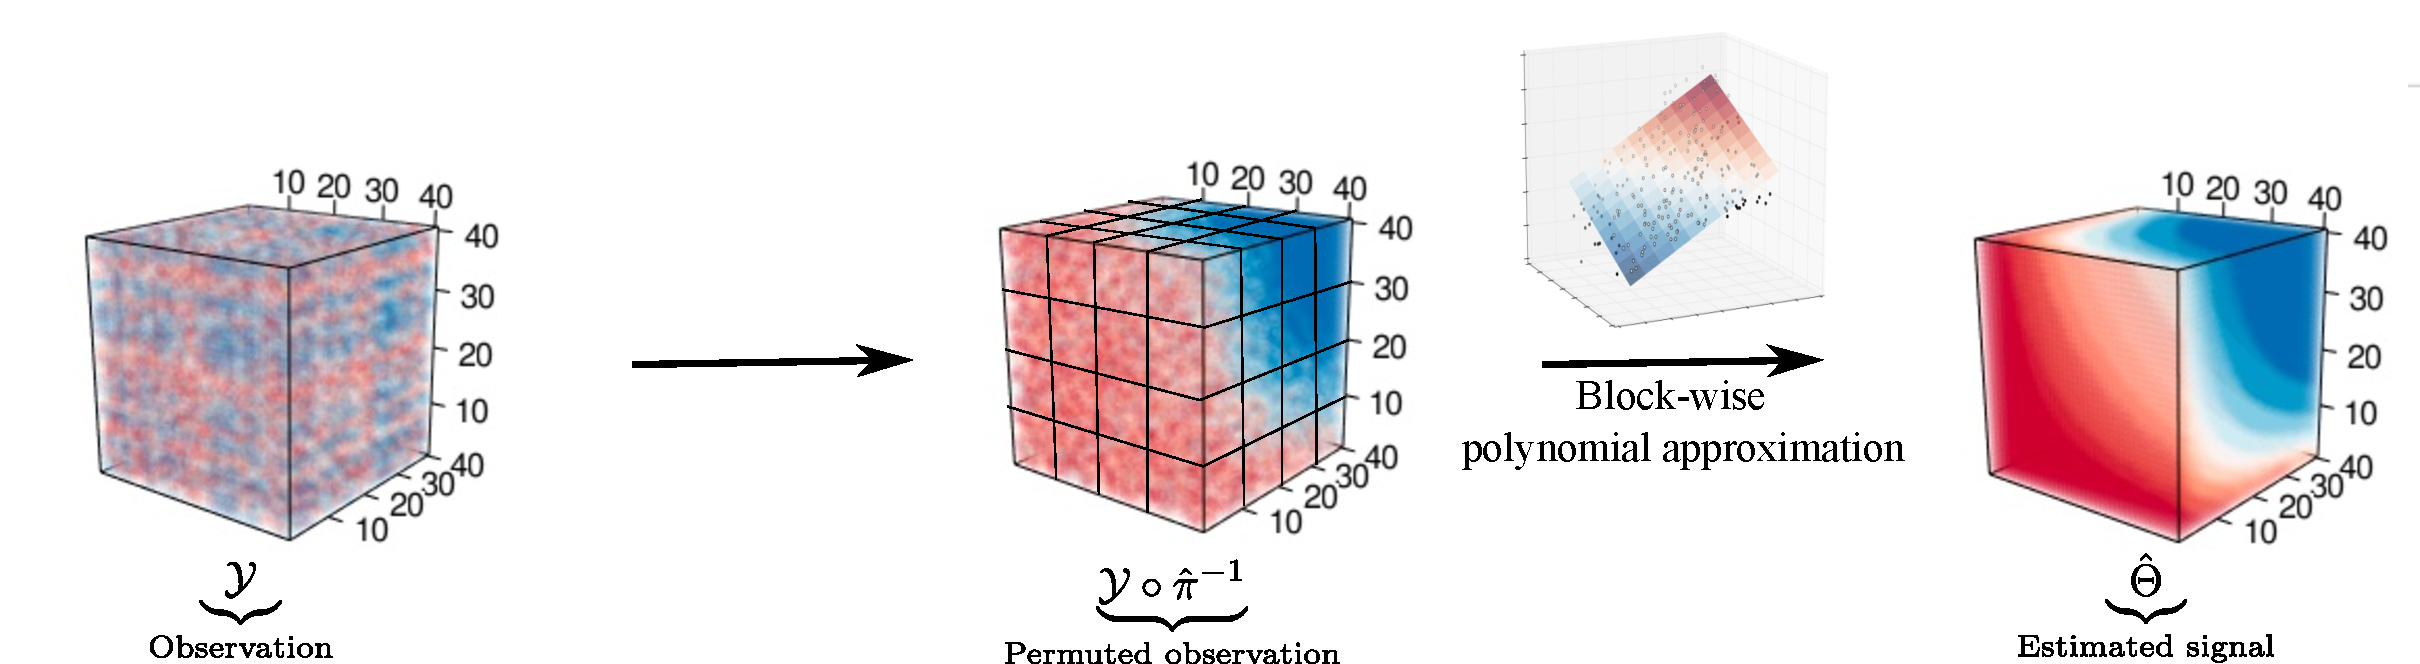
\includegraphics[width = \textwidth]{figure/estm.pdf}
\end{figure}
\onslide<2->{
 \begin{itemize}
\item We propose the {\color{red}least square estimation},
\begin{align}\label{eq:lseopt}
    (\hat\Theta^{\text{LSE}},&\hat \pi^{\text{LSE}}) = \argmin_{\Theta\in\caliB(k,\ell), \  \pi\in [d]\to[d]}\FnormSize{}{\tY-\Theta\circ\pi}\quad \text{ where,} \\&\scalebox{0.9}{$\caliB(k,\ell) = \bigg\{\tB\in(\mathbb{R}^d)^{\otimes m}\colon \tB(\omega) = \sum_{\Delta\in\tE_k}\text{Poly}_{\ell,\Delta}(\omega)\mathds{1}\{\omega\in\Delta\}\text{ for all } \omega\in[d]^m\bigg\}.$}
\end{align}
\end{itemize}
}
\end{frame}



\begin{frame}{Least-squares estimation error and its optimality}
For two tensor $\Theta_1,\Theta_2$, define $\textup{MSE}(\Theta_1,\Theta_2) = \frac{1}{d^m}\FnormSize{}{\Theta_1-\Theta_2}^2.$
    \begin{block}{Least-squares estimation error (L. and Wang 2021)}
    Suppose that the generating function $f$ is $\alpha$-H\"older smooth. 
  For optimally chosen polynomial degree $\ell^*$ and the number of groups $k^*$,
\begin{align}\label{eq:rateMSE}
\textup{MSE}(\hat\Theta^{\textup{LSE}}\circ\hat\pi^{\textup{LSE}},\Theta\circ\pi)\lesssim  \begin{cases}{\color{Fuchsia}d^{-{2m\alpha\over m+2\alpha}}} & \text{ when } \alpha < \frac{m(m-1)}{2},\\{\color{MidnightBlue}\log d\over d^{m-1}}&\text{ when } \alpha \geq \frac{m(m-1)}{2}.\end{cases}
\end{align}
% \item For any given $\alpha\in(0,\infty)$,  the estimation problem obeys the minimax lower bound, 
% \begin{equation}\label{eq:minimax}
% \inf_{(\hat \Theta,\hat \pi)}\sup_{f\in \tH(\alpha), \pi\in[d]\to[d]} \mathbb{P}\left(\textup{MSE}(\hat\Theta\circ\hat\pi,\ \Theta\circ\pi) \gtrsim {\color{red}d^{-{2m\alpha\over m+2\alpha}}}+{\color{blue}\frac{\log d}{d^{m-1}}} \right) \geq 0.8.
% \end{equation}
 
    \end{block}
    \vspace{-0.2cm}
    {\scriptsize\hfill $\ell^* = \min(\lceil\alpha\rceil,m(m-1)/2)-1 $ and $k^* = \lceil  d^{m/ (m+2\min(\alpha,\ell^*+1))}\rceil$}

    \begin{itemize}
        \item The error consists of the {\color{Fuchsia}nonparametric error } and {\color{MidnightBlue} permutation error.} 
        \item The dominating error depends on {\color{red}the smoothness and order of tensor}.
        \item We show that the least-square estimation is {\color{red}minimax rate-optimal}.
    \end{itemize}

\onslide<2->{    
However, the algorithm for the least square estimation is {\color{red}computationally intractable}. }
\end{frame}


\begin{frame}{Polynomial-time algorithm: Borda count estimation}
\begin{enumerate}
  \item {\bf Sorting stage}: Estimate a permutation $\hat\pi^{\text{BC}}$  such that the permuted score function $\tau\circ (\hat\pi^{\text{BC}})^{-1}$ is monotonically increasing, where \[\tau(i) = \frac{1}{d^{m-1}}\sum_{(i_2,\ldots,i_m)\in[d]^{m-1}} \tY(i,i_2,\ldots,i_m).\] 
 \item {\bf Polynomial approximation stage}: Estimate the degree-$\ell$ polynomial block tensor
    \begin{align}\label{eq:bclse}
        \hat\Theta^{\text{BC}} = \argmin_{\Theta\in\caliB(k,\ell)}\FnormSize{}{\tY\circ(\hat\pi^{\text{BC}})^{-1}-\Theta}.
    \end{align}
    \end{enumerate}
\vspace{-.5cm}
\onslide<2->{
\begin{figure}
    \centering
    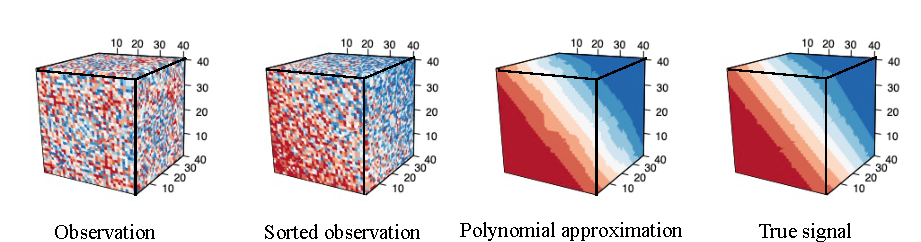
\includegraphics[width = 0.8\textwidth]{figure/Borda.pdf}
\end{figure}

Borda count algorithm provably achieves {\color{red}optimal rate} under {\color{red}monotonicity assumptions}
}
\end{frame}

\begin{frame}{Simulation results}
\begin{figure}
    \centering
    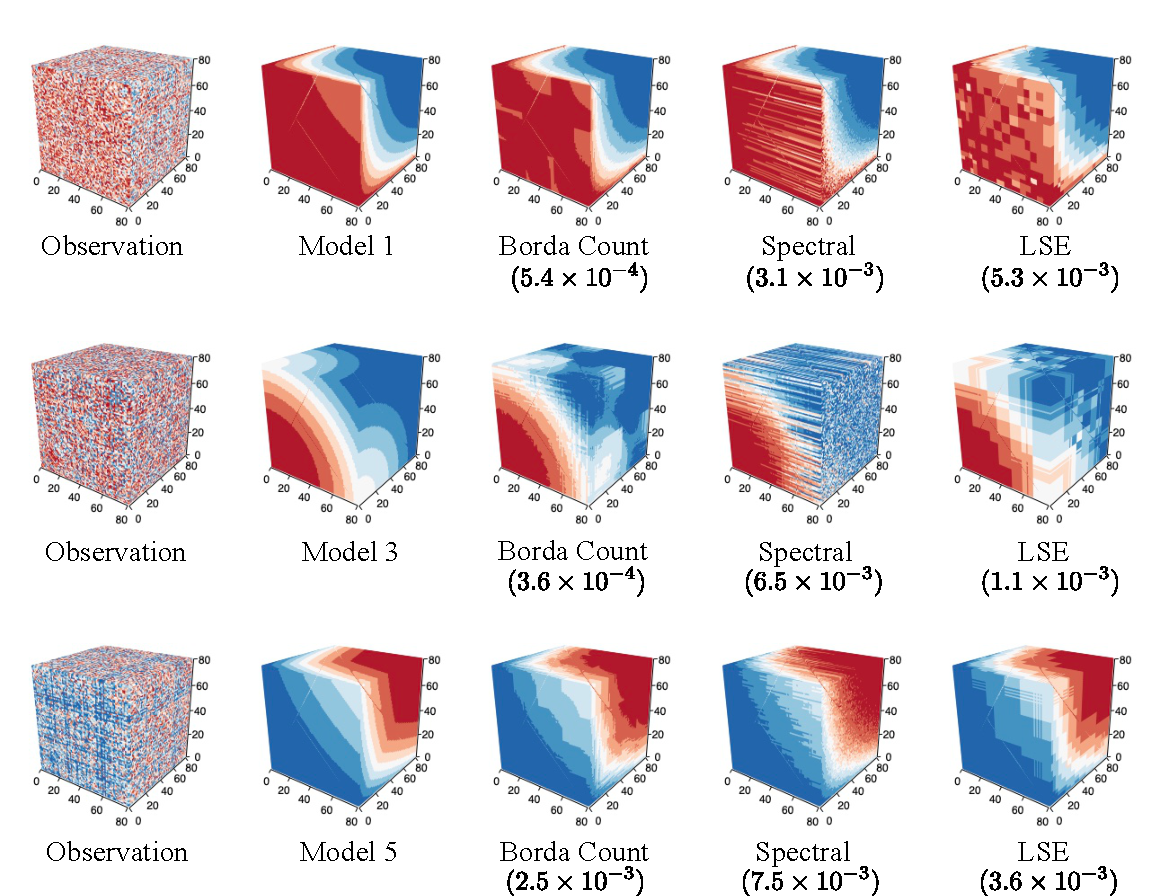
\includegraphics[width = 10cm]{figure/vfinal.pdf}
    \caption{Caption}
    \label{fig:my_label}
\end{figure}
    
\end{frame}


\begin{frame}
    \Huge{\centerline{Thank you!}}
\end{frame}
% \begin{frame}{Conclusion}
%         \begin{itemize}
% \item We have developed permuted smooth tensor model and estimation methods via {\color{red}block-wise polynomial approximation}.
% \item We show that the least square estimation achieves the {\color{red}minimax optimal rate}.
% \item  We provide the {\color{red}polynomial-time Borda count algorithm}  with the same convergence rate under monotonicity conditions.
% %An optimal error bound for the least square estimation is established based on block-wise polynomial approximation. Borda count estimation with polynomial algorithm is provided with the same convergence rate under $\beta$-monotonicity. 
% \item Numerical analysis in the main paper demonstrates the performance and applicability of our method.
% \end{itemize}
% \end{frame}




\appendix
% \begin{frame}{Appendix: algorithm}\label{algorithm}
% \hfill\hyperlink{weighted}{\beamerbutton{back}}
% \includegraphics[width = \textwidth]{figure/algorithm.pdf}

% \end{frame}


\begin{frame}[allowframebreaks]
        \frametitle{References}
\bibliographystyle{apalike} 
\bibliography{tensor_wang}
\end{frame}

%------------------------------------------------

%----------------------------------------------------------------------------------------

\end{document}
